\documentclass[twoside]{book}

% Packages required by doxygen
\usepackage{calc}
\usepackage{doxygen}
\usepackage{graphicx}
\usepackage[utf8]{inputenc}
\usepackage{makeidx}
\usepackage{multicol}
\usepackage{multirow}
\usepackage{textcomp}
\usepackage[table]{xcolor}

% Font selection
\usepackage[T1]{fontenc}
\usepackage{mathptmx}
\usepackage[scaled=.90]{helvet}
\usepackage{courier}
\usepackage{amssymb}
\usepackage{sectsty}
\renewcommand{\familydefault}{\sfdefault}
\allsectionsfont{%
  \fontseries{bc}\selectfont%
  \color{darkgray}%
}
\renewcommand{\DoxyLabelFont}{%
  \fontseries{bc}\selectfont%
  \color{darkgray}%
}

% Page & text layout
\usepackage{geometry}
\geometry{%
  a4paper,%
  top=2.5cm,%
  bottom=2.5cm,%
  left=2.5cm,%
  right=2.5cm%
}
\tolerance=750
\hfuzz=15pt
\hbadness=750
\setlength{\emergencystretch}{15pt}
\setlength{\parindent}{0cm}
\setlength{\parskip}{0.2cm}
\makeatletter
\renewcommand{\paragraph}{%
  \@startsection{paragraph}{4}{0ex}{-1.0ex}{1.0ex}{%
    \normalfont\normalsize\bfseries\SS@parafont%
  }%
}
\renewcommand{\subparagraph}{%
  \@startsection{subparagraph}{5}{0ex}{-1.0ex}{1.0ex}{%
    \normalfont\normalsize\bfseries\SS@subparafont%
  }%
}
\makeatother

% Headers & footers
\usepackage{fancyhdr}
\pagestyle{fancyplain}
\fancyhead[LE]{\fancyplain{}{\bfseries\thepage}}
\fancyhead[CE]{\fancyplain{}{}}
\fancyhead[RE]{\fancyplain{}{\bfseries\leftmark}}
\fancyhead[LO]{\fancyplain{}{\bfseries\rightmark}}
\fancyhead[CO]{\fancyplain{}{}}
\fancyhead[RO]{\fancyplain{}{\bfseries\thepage}}
\fancyfoot[LE]{\fancyplain{}{}}
\fancyfoot[CE]{\fancyplain{}{}}
\fancyfoot[RE]{\fancyplain{}{\bfseries\scriptsize Generated on Mon Feb 5 2018 09\-:33\-:57 for My Project by Doxygen }}
\fancyfoot[LO]{\fancyplain{}{\bfseries\scriptsize Generated on Mon Feb 5 2018 09\-:33\-:57 for My Project by Doxygen }}
\fancyfoot[CO]{\fancyplain{}{}}
\fancyfoot[RO]{\fancyplain{}{}}
\renewcommand{\footrulewidth}{0.4pt}
\renewcommand{\chaptermark}[1]{%
  \markboth{#1}{}%
}
\renewcommand{\sectionmark}[1]{%
  \markright{\thesection\ #1}%
}

% Indices & bibliography
\usepackage{natbib}
\usepackage[titles]{tocloft}
\setcounter{tocdepth}{3}
\setcounter{secnumdepth}{5}
\makeindex

% Hyperlinks (required, but should be loaded last)
\usepackage{ifpdf}
\ifpdf
  \usepackage[pdftex,pagebackref=true]{hyperref}
\else
  \usepackage[ps2pdf,pagebackref=true]{hyperref}
\fi
\hypersetup{%
  colorlinks=true,%
  linkcolor=blue,%
  citecolor=blue,%
  unicode%
}

% Custom commands
\newcommand{\clearemptydoublepage}{%
  \newpage{\pagestyle{empty}\cleardoublepage}%
}


%===== C O N T E N T S =====

\begin{document}

% Titlepage & ToC
\hypersetup{pageanchor=false}
\pagenumbering{roman}
\begin{titlepage}
\vspace*{7cm}
\begin{center}%
{\Large My Project }\\
\vspace*{1cm}
{\large Generated by Doxygen 1.8.6}\\
\vspace*{0.5cm}
{\small Mon Feb 5 2018 09:33:57}\\
\end{center}
\end{titlepage}
\clearemptydoublepage
\tableofcontents
\clearemptydoublepage
\pagenumbering{arabic}
\hypersetup{pageanchor=true}

%--- Begin generated contents ---
\chapter{Hierarchical Index}
\section{Class Hierarchy}
This inheritance list is sorted roughly, but not completely, alphabetically\-:\begin{DoxyCompactList}
\item \contentsline{section}{Command}{\pageref{class_command}}{}
\begin{DoxyCompactList}
\item \contentsline{section}{Create\-Document\-Command}{\pageref{class_create_document_command}}{}
\item \contentsline{section}{Create\-Shape\-Command}{\pageref{class_create_shape_command}}{}
\item \contentsline{section}{Delete\-Shape\-Command}{\pageref{class_delete_shape_command}}{}
\item \contentsline{section}{Open\-Document\-Command}{\pageref{class_open_document_command}}{}
\item \contentsline{section}{Save\-As\-Document\-Command}{\pageref{class_save_as_document_command}}{}
\item \contentsline{section}{Save\-Document\-Command}{\pageref{class_save_document_command}}{}
\end{DoxyCompactList}
\item \contentsline{section}{Document}{\pageref{class_document}}{}
\item \contentsline{section}{Graph\-Editor}{\pageref{class_graph_editor}}{}
\item \contentsline{section}{Shape}{\pageref{class_shape}}{}
\begin{DoxyCompactList}
\item \contentsline{section}{Circle}{\pageref{class_circle}}{}
\item \contentsline{section}{Rectangle}{\pageref{class_rectangle}}{}
\end{DoxyCompactList}
\end{DoxyCompactList}

\chapter{Class Index}
\section{Class List}
Here are the classes, structs, unions and interfaces with brief descriptions\-:\begin{DoxyCompactList}
\item\contentsline{section}{\hyperlink{classis__container}{is\-\_\-container$<$ T $>$} }{\pageref{classis__container}}{}
\item\contentsline{section}{\hyperlink{structiterate__tuple}{iterate\-\_\-tuple$<$ is\-\_\-same\-\_\-type, index, Printer, Args $>$} }{\pageref{structiterate__tuple}}{}
\item\contentsline{section}{\hyperlink{structiterate__tuple_3_01false_00_01index_00_01_printer_00_01_args_8_8_8_4}{iterate\-\_\-tuple$<$ false, index, Printer, Args...$>$} }{\pageref{structiterate__tuple_3_01false_00_01index_00_01_printer_00_01_args_8_8_8_4}}{}
\item\contentsline{section}{\hyperlink{structiterate__tuple_3_01state_00_010_00_01_printer_00_01_args_8_8_8_4}{iterate\-\_\-tuple$<$ state, 0, Printer, Args...$>$} }{\pageref{structiterate__tuple_3_01state_00_010_00_01_printer_00_01_args_8_8_8_4}}{}
\item\contentsline{section}{\hyperlink{structt__printer}{t\-\_\-printer} }{\pageref{structt__printer}}{}
\end{DoxyCompactList}

\chapter{File Index}
\section{File List}
Here is a list of all files with brief descriptions\-:\begin{DoxyCompactList}
\item\contentsline{section}{\hyperlink{document_8h}{document.\-h} }{\pageref{document_8h}}{}
\item\contentsline{section}{\hyperlink{main_8cpp}{main.\-cpp} }{\pageref{main_8cpp}}{}
\item\contentsline{section}{\hyperlink{shape_8h}{shape.\-h} }{\pageref{shape_8h}}{}
\item\contentsline{section}{\hyperlink{version_8h}{version.\-h} }{\pageref{version_8h}}{}
\end{DoxyCompactList}

\chapter{Class Documentation}
\hypertarget{class_circle}{\section{Circle Class Reference}
\label{class_circle}\index{Circle@{Circle}}
}


{\ttfamily \#include $<$shape.\-h$>$}



Inheritance diagram for Circle\-:
\nopagebreak
\begin{figure}[H]
\begin{center}
\leavevmode
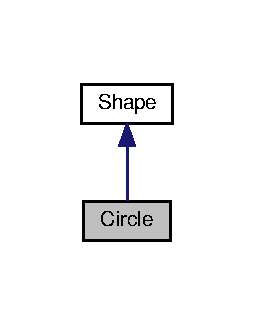
\includegraphics[width=122pt]{class_circle__inherit__graph}
\end{center}
\end{figure}


Collaboration diagram for Circle\-:
\nopagebreak
\begin{figure}[H]
\begin{center}
\leavevmode
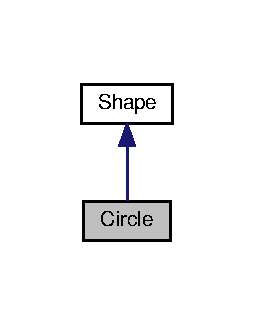
\includegraphics[width=122pt]{class_circle__coll__graph}
\end{center}
\end{figure}
\subsection*{Public Member Functions}
\begin{DoxyCompactItemize}
\item 
\hyperlink{class_circle}{Circle} \& \hyperlink{class_circle_acbb38b1159540be80700263d78a9805e}{Create} () override
\item 
void \hyperlink{class_circle_aef290a1d0349f56cb01884b6735042cb}{Delete} () override
\end{DoxyCompactItemize}
\subsection*{Additional Inherited Members}


\subsection{Member Function Documentation}
\hypertarget{class_circle_acbb38b1159540be80700263d78a9805e}{\index{Circle@{Circle}!Create@{Create}}
\index{Create@{Create}!Circle@{Circle}}
\subsubsection[{Create}]{\setlength{\rightskip}{0pt plus 5cm}{\bf Circle}\& Circle\-::\-Create (
\begin{DoxyParamCaption}
{}
\end{DoxyParamCaption}
)\hspace{0.3cm}{\ttfamily [inline]}, {\ttfamily [override]}, {\ttfamily [virtual]}}}\label{class_circle_acbb38b1159540be80700263d78a9805e}


Implements \hyperlink{class_shape_ad2be0ce227fb05dcfec2691a671c82b5}{Shape}.

\hypertarget{class_circle_aef290a1d0349f56cb01884b6735042cb}{\index{Circle@{Circle}!Delete@{Delete}}
\index{Delete@{Delete}!Circle@{Circle}}
\subsubsection[{Delete}]{\setlength{\rightskip}{0pt plus 5cm}void Circle\-::\-Delete (
\begin{DoxyParamCaption}
{}
\end{DoxyParamCaption}
)\hspace{0.3cm}{\ttfamily [inline]}, {\ttfamily [override]}, {\ttfamily [virtual]}}}\label{class_circle_aef290a1d0349f56cb01884b6735042cb}


Implements \hyperlink{class_shape_a03a2b4615053e0a0edbdc42283e0bb04}{Shape}.



The documentation for this class was generated from the following file\-:\begin{DoxyCompactItemize}
\item 
\hyperlink{shape_8h}{shape.\-h}\end{DoxyCompactItemize}

\hypertarget{class_command}{\section{Command Class Reference}
\label{class_command}\index{Command@{Command}}
}


Inheritance diagram for Command\-:
\nopagebreak
\begin{figure}[H]
\begin{center}
\leavevmode
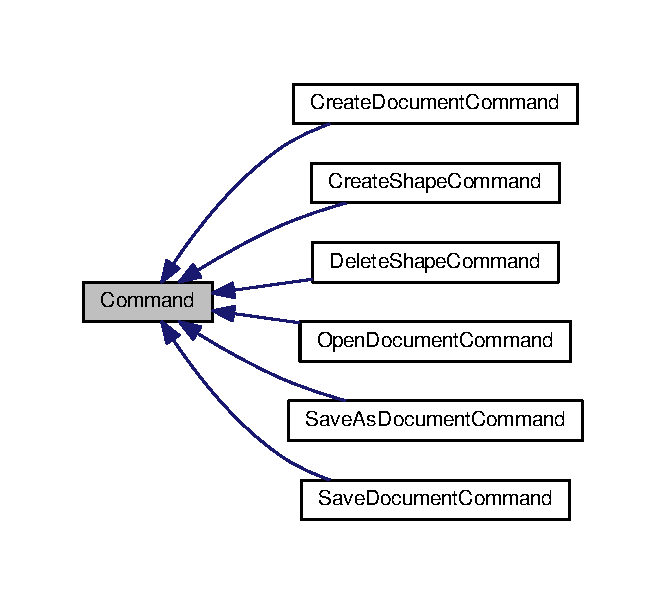
\includegraphics[width=320pt]{class_command__inherit__graph}
\end{center}
\end{figure}


Collaboration diagram for Command\-:
\nopagebreak
\begin{figure}[H]
\begin{center}
\leavevmode
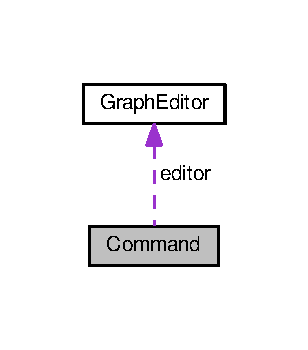
\includegraphics[width=148pt]{class_command__coll__graph}
\end{center}
\end{figure}
\subsection*{Public Member Functions}
\begin{DoxyCompactItemize}
\item 
virtual void \hyperlink{class_command_a6fd7d9bd8df8bfc881e4d6c7cd1878b7}{execute} ()=0
\item 
virtual \hyperlink{class_command_aa545a53d35818f9efb936daf3fa16c61}{$\sim$\-Command} ()=default
\end{DoxyCompactItemize}
\subsection*{Protected Member Functions}
\begin{DoxyCompactItemize}
\item 
\hyperlink{class_command_af128b983a5de6ebb74c4da60cc5d5e24}{Command} (\hyperlink{class_graph_editor}{Graph\-Editor} $\ast$g)
\end{DoxyCompactItemize}
\subsection*{Protected Attributes}
\begin{DoxyCompactItemize}
\item 
\hyperlink{class_graph_editor}{Graph\-Editor} $\ast$ \hyperlink{class_command_a2803422581a3f0c430cdfdcaf2f0e99f}{editor}
\end{DoxyCompactItemize}


\subsection{Constructor \& Destructor Documentation}
\hypertarget{class_command_aa545a53d35818f9efb936daf3fa16c61}{\index{Command@{Command}!$\sim$\-Command@{$\sim$\-Command}}
\index{$\sim$\-Command@{$\sim$\-Command}!Command@{Command}}
\subsubsection[{$\sim$\-Command}]{\setlength{\rightskip}{0pt plus 5cm}virtual Command\-::$\sim$\-Command (
\begin{DoxyParamCaption}
{}
\end{DoxyParamCaption}
)\hspace{0.3cm}{\ttfamily [virtual]}, {\ttfamily [default]}}}\label{class_command_aa545a53d35818f9efb936daf3fa16c61}
\hypertarget{class_command_af128b983a5de6ebb74c4da60cc5d5e24}{\index{Command@{Command}!Command@{Command}}
\index{Command@{Command}!Command@{Command}}
\subsubsection[{Command}]{\setlength{\rightskip}{0pt plus 5cm}Command\-::\-Command (
\begin{DoxyParamCaption}
\item[{{\bf Graph\-Editor} $\ast$}]{g}
\end{DoxyParamCaption}
)\hspace{0.3cm}{\ttfamily [inline]}, {\ttfamily [protected]}}}\label{class_command_af128b983a5de6ebb74c4da60cc5d5e24}


\subsection{Member Function Documentation}
\hypertarget{class_command_a6fd7d9bd8df8bfc881e4d6c7cd1878b7}{\index{Command@{Command}!execute@{execute}}
\index{execute@{execute}!Command@{Command}}
\subsubsection[{execute}]{\setlength{\rightskip}{0pt plus 5cm}virtual void Command\-::execute (
\begin{DoxyParamCaption}
{}
\end{DoxyParamCaption}
)\hspace{0.3cm}{\ttfamily [pure virtual]}}}\label{class_command_a6fd7d9bd8df8bfc881e4d6c7cd1878b7}


Implemented in \hyperlink{class_delete_shape_command_abbd59d12e3addf806275a6a0bde75456}{Delete\-Shape\-Command}, \hyperlink{class_create_shape_command_af855704915f8a27d3c3573de67fb546e}{Create\-Shape\-Command}, \hyperlink{class_save_as_document_command_a7e24e4880ba0d3545f3df16ef5116d40}{Save\-As\-Document\-Command}, \hyperlink{class_save_document_command_a2c3e0a729f64b2577ed201cf20395895}{Save\-Document\-Command}, \hyperlink{class_open_document_command_a80a9aa7d2c61e149c87800998f22f0ea}{Open\-Document\-Command}, and \hyperlink{class_create_document_command_abbdce229ede2849547c17b4f0e5c42f5}{Create\-Document\-Command}.



\subsection{Member Data Documentation}
\hypertarget{class_command_a2803422581a3f0c430cdfdcaf2f0e99f}{\index{Command@{Command}!editor@{editor}}
\index{editor@{editor}!Command@{Command}}
\subsubsection[{editor}]{\setlength{\rightskip}{0pt plus 5cm}{\bf Graph\-Editor}$\ast$ Command\-::editor\hspace{0.3cm}{\ttfamily [protected]}}}\label{class_command_a2803422581a3f0c430cdfdcaf2f0e99f}


The documentation for this class was generated from the following file\-:\begin{DoxyCompactItemize}
\item 
\hyperlink{main_8cpp}{main.\-cpp}\end{DoxyCompactItemize}

\hypertarget{class_create_document_command}{\section{Create\-Document\-Command Class Reference}
\label{class_create_document_command}\index{Create\-Document\-Command@{Create\-Document\-Command}}
}


Inheritance diagram for Create\-Document\-Command\-:
\nopagebreak
\begin{figure}[H]
\begin{center}
\leavevmode
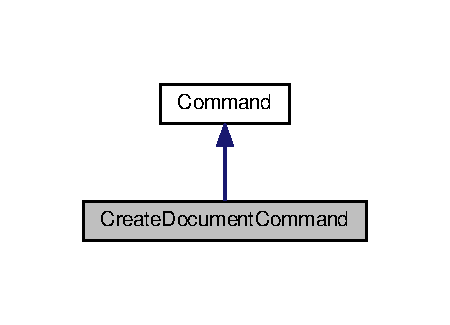
\includegraphics[width=216pt]{class_create_document_command__inherit__graph}
\end{center}
\end{figure}


Collaboration diagram for Create\-Document\-Command\-:
\nopagebreak
\begin{figure}[H]
\begin{center}
\leavevmode
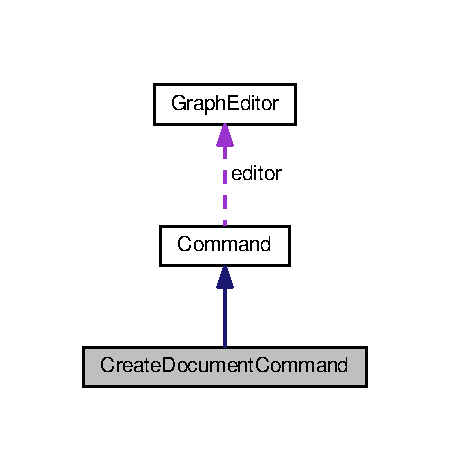
\includegraphics[width=216pt]{class_create_document_command__coll__graph}
\end{center}
\end{figure}
\subsection*{Public Member Functions}
\begin{DoxyCompactItemize}
\item 
\hyperlink{class_create_document_command_a8372d0b0f0d1eeeb87a373654644d64e}{Create\-Document\-Command} (\hyperlink{class_graph_editor}{Graph\-Editor} $\ast$g)
\item 
void \hyperlink{class_create_document_command_abbdce229ede2849547c17b4f0e5c42f5}{execute} () override
\end{DoxyCompactItemize}
\subsection*{Additional Inherited Members}


\subsection{Constructor \& Destructor Documentation}
\hypertarget{class_create_document_command_a8372d0b0f0d1eeeb87a373654644d64e}{\index{Create\-Document\-Command@{Create\-Document\-Command}!Create\-Document\-Command@{Create\-Document\-Command}}
\index{Create\-Document\-Command@{Create\-Document\-Command}!CreateDocumentCommand@{Create\-Document\-Command}}
\subsubsection[{Create\-Document\-Command}]{\setlength{\rightskip}{0pt plus 5cm}Create\-Document\-Command\-::\-Create\-Document\-Command (
\begin{DoxyParamCaption}
\item[{{\bf Graph\-Editor} $\ast$}]{g}
\end{DoxyParamCaption}
)\hspace{0.3cm}{\ttfamily [inline]}}}\label{class_create_document_command_a8372d0b0f0d1eeeb87a373654644d64e}


\subsection{Member Function Documentation}
\hypertarget{class_create_document_command_abbdce229ede2849547c17b4f0e5c42f5}{\index{Create\-Document\-Command@{Create\-Document\-Command}!execute@{execute}}
\index{execute@{execute}!CreateDocumentCommand@{Create\-Document\-Command}}
\subsubsection[{execute}]{\setlength{\rightskip}{0pt plus 5cm}void Create\-Document\-Command\-::execute (
\begin{DoxyParamCaption}
{}
\end{DoxyParamCaption}
)\hspace{0.3cm}{\ttfamily [inline]}, {\ttfamily [override]}, {\ttfamily [virtual]}}}\label{class_create_document_command_abbdce229ede2849547c17b4f0e5c42f5}


Implements \hyperlink{class_command_a6fd7d9bd8df8bfc881e4d6c7cd1878b7}{Command}.



The documentation for this class was generated from the following file\-:\begin{DoxyCompactItemize}
\item 
\hyperlink{main_8cpp}{main.\-cpp}\end{DoxyCompactItemize}

\hypertarget{class_create_shape_command}{\section{Create\-Shape\-Command Class Reference}
\label{class_create_shape_command}\index{Create\-Shape\-Command@{Create\-Shape\-Command}}
}


Inheritance diagram for Create\-Shape\-Command\-:
\nopagebreak
\begin{figure}[H]
\begin{center}
\leavevmode
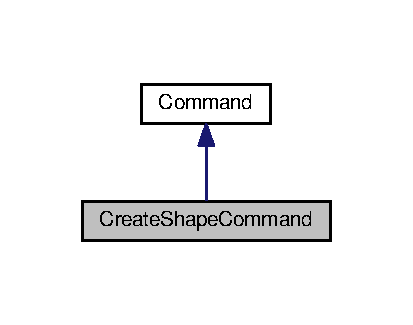
\includegraphics[width=198pt]{class_create_shape_command__inherit__graph}
\end{center}
\end{figure}


Collaboration diagram for Create\-Shape\-Command\-:
\nopagebreak
\begin{figure}[H]
\begin{center}
\leavevmode
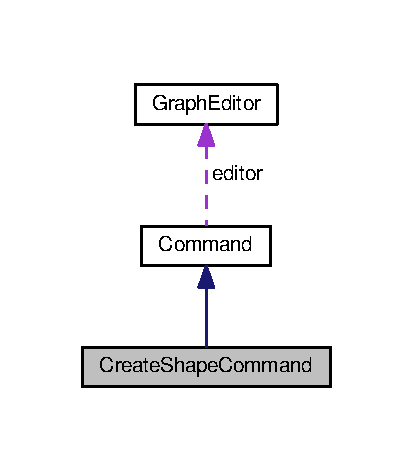
\includegraphics[width=198pt]{class_create_shape_command__coll__graph}
\end{center}
\end{figure}
\subsection*{Public Member Functions}
\begin{DoxyCompactItemize}
\item 
\hyperlink{class_create_shape_command_a19f4bf474cc3f7960294e56c06fc51b9}{Create\-Shape\-Command} (\hyperlink{class_graph_editor}{Graph\-Editor} $\ast$g, \hyperlink{class_shape}{Shape} $\ast$s)
\item 
void \hyperlink{class_create_shape_command_af855704915f8a27d3c3573de67fb546e}{execute} () override
\end{DoxyCompactItemize}
\subsection*{Additional Inherited Members}


\subsection{Constructor \& Destructor Documentation}
\hypertarget{class_create_shape_command_a19f4bf474cc3f7960294e56c06fc51b9}{\index{Create\-Shape\-Command@{Create\-Shape\-Command}!Create\-Shape\-Command@{Create\-Shape\-Command}}
\index{Create\-Shape\-Command@{Create\-Shape\-Command}!CreateShapeCommand@{Create\-Shape\-Command}}
\subsubsection[{Create\-Shape\-Command}]{\setlength{\rightskip}{0pt plus 5cm}Create\-Shape\-Command\-::\-Create\-Shape\-Command (
\begin{DoxyParamCaption}
\item[{{\bf Graph\-Editor} $\ast$}]{g, }
\item[{{\bf Shape} $\ast$}]{s}
\end{DoxyParamCaption}
)\hspace{0.3cm}{\ttfamily [inline]}}}\label{class_create_shape_command_a19f4bf474cc3f7960294e56c06fc51b9}


\subsection{Member Function Documentation}
\hypertarget{class_create_shape_command_af855704915f8a27d3c3573de67fb546e}{\index{Create\-Shape\-Command@{Create\-Shape\-Command}!execute@{execute}}
\index{execute@{execute}!CreateShapeCommand@{Create\-Shape\-Command}}
\subsubsection[{execute}]{\setlength{\rightskip}{0pt plus 5cm}void Create\-Shape\-Command\-::execute (
\begin{DoxyParamCaption}
{}
\end{DoxyParamCaption}
)\hspace{0.3cm}{\ttfamily [inline]}, {\ttfamily [override]}, {\ttfamily [virtual]}}}\label{class_create_shape_command_af855704915f8a27d3c3573de67fb546e}


Implements \hyperlink{class_command_a6fd7d9bd8df8bfc881e4d6c7cd1878b7}{Command}.



The documentation for this class was generated from the following file\-:\begin{DoxyCompactItemize}
\item 
\hyperlink{main_8cpp}{main.\-cpp}\end{DoxyCompactItemize}

\hypertarget{class_delete_shape_command}{\section{Delete\-Shape\-Command Class Reference}
\label{class_delete_shape_command}\index{Delete\-Shape\-Command@{Delete\-Shape\-Command}}
}


Inheritance diagram for Delete\-Shape\-Command\-:
\nopagebreak
\begin{figure}[H]
\begin{center}
\leavevmode
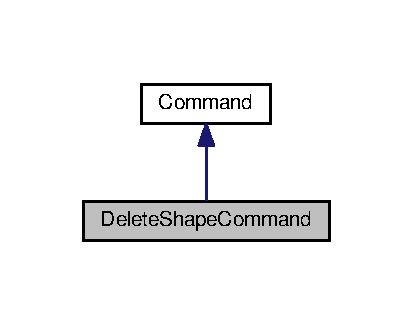
\includegraphics[width=198pt]{class_delete_shape_command__inherit__graph}
\end{center}
\end{figure}


Collaboration diagram for Delete\-Shape\-Command\-:
\nopagebreak
\begin{figure}[H]
\begin{center}
\leavevmode
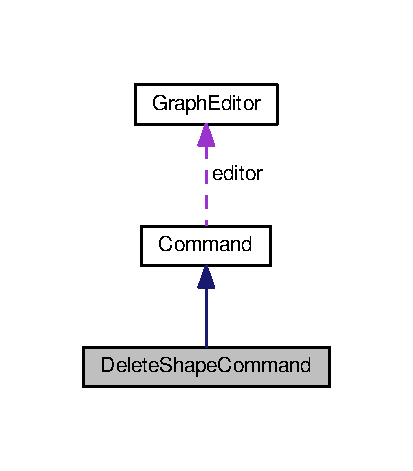
\includegraphics[width=198pt]{class_delete_shape_command__coll__graph}
\end{center}
\end{figure}
\subsection*{Public Member Functions}
\begin{DoxyCompactItemize}
\item 
\hyperlink{class_delete_shape_command_ac56ba7e4a163ba613cd2e5e186fc092c}{Delete\-Shape\-Command} (\hyperlink{class_graph_editor}{Graph\-Editor} $\ast$g, \hyperlink{class_shape}{Shape} $\ast$s)
\item 
void \hyperlink{class_delete_shape_command_abbd59d12e3addf806275a6a0bde75456}{execute} () override
\end{DoxyCompactItemize}
\subsection*{Additional Inherited Members}


\subsection{Constructor \& Destructor Documentation}
\hypertarget{class_delete_shape_command_ac56ba7e4a163ba613cd2e5e186fc092c}{\index{Delete\-Shape\-Command@{Delete\-Shape\-Command}!Delete\-Shape\-Command@{Delete\-Shape\-Command}}
\index{Delete\-Shape\-Command@{Delete\-Shape\-Command}!DeleteShapeCommand@{Delete\-Shape\-Command}}
\subsubsection[{Delete\-Shape\-Command}]{\setlength{\rightskip}{0pt plus 5cm}Delete\-Shape\-Command\-::\-Delete\-Shape\-Command (
\begin{DoxyParamCaption}
\item[{{\bf Graph\-Editor} $\ast$}]{g, }
\item[{{\bf Shape} $\ast$}]{s}
\end{DoxyParamCaption}
)\hspace{0.3cm}{\ttfamily [inline]}}}\label{class_delete_shape_command_ac56ba7e4a163ba613cd2e5e186fc092c}


\subsection{Member Function Documentation}
\hypertarget{class_delete_shape_command_abbd59d12e3addf806275a6a0bde75456}{\index{Delete\-Shape\-Command@{Delete\-Shape\-Command}!execute@{execute}}
\index{execute@{execute}!DeleteShapeCommand@{Delete\-Shape\-Command}}
\subsubsection[{execute}]{\setlength{\rightskip}{0pt plus 5cm}void Delete\-Shape\-Command\-::execute (
\begin{DoxyParamCaption}
{}
\end{DoxyParamCaption}
)\hspace{0.3cm}{\ttfamily [inline]}, {\ttfamily [override]}, {\ttfamily [virtual]}}}\label{class_delete_shape_command_abbd59d12e3addf806275a6a0bde75456}


Implements \hyperlink{class_command_a6fd7d9bd8df8bfc881e4d6c7cd1878b7}{Command}.



The documentation for this class was generated from the following file\-:\begin{DoxyCompactItemize}
\item 
\hyperlink{main_8cpp}{main.\-cpp}\end{DoxyCompactItemize}

\hypertarget{class_document}{\section{Document Class Reference}
\label{class_document}\index{Document@{Document}}
}


{\ttfamily \#include $<$document.\-h$>$}

\subsection*{Public Member Functions}
\begin{DoxyCompactItemize}
\item 
\hyperlink{class_document_acdbcbe550084e8c20f4f67eb229ad66a}{Document} ()
\item 
void \hyperlink{class_document_a84c4301459df072670d66a1792c702ef}{Open} (std\-::string name)
\item 
void \hyperlink{class_document_ac09705578d294172c64c8a8cd627306f}{Save} ()
\item 
void \hyperlink{class_document_ae070257ab792b45432b2cbfafe6a2c3b}{Save\-As\-Document} (std\-::string new\-\_\-name)
\item 
void \hyperlink{class_document_ab1f52696ee2c852463e08ad24b52230f}{Create\-Shape} (\hyperlink{class_shape}{Shape} $\ast$shape)
\item 
void \hyperlink{class_document_a7947653edee614668954b9a2b5fc0b51}{Delete\-Shape} (\hyperlink{class_shape}{Shape} $\ast$shape)
\end{DoxyCompactItemize}


\subsection{Constructor \& Destructor Documentation}
\hypertarget{class_document_acdbcbe550084e8c20f4f67eb229ad66a}{\index{Document@{Document}!Document@{Document}}
\index{Document@{Document}!Document@{Document}}
\subsubsection[{Document}]{\setlength{\rightskip}{0pt plus 5cm}Document\-::\-Document (
\begin{DoxyParamCaption}
{}
\end{DoxyParamCaption}
)\hspace{0.3cm}{\ttfamily [inline]}}}\label{class_document_acdbcbe550084e8c20f4f67eb229ad66a}


\subsection{Member Function Documentation}
\hypertarget{class_document_ab1f52696ee2c852463e08ad24b52230f}{\index{Document@{Document}!Create\-Shape@{Create\-Shape}}
\index{Create\-Shape@{Create\-Shape}!Document@{Document}}
\subsubsection[{Create\-Shape}]{\setlength{\rightskip}{0pt plus 5cm}void Document\-::\-Create\-Shape (
\begin{DoxyParamCaption}
\item[{{\bf Shape} $\ast$}]{shape}
\end{DoxyParamCaption}
)\hspace{0.3cm}{\ttfamily [inline]}}}\label{class_document_ab1f52696ee2c852463e08ad24b52230f}
\hypertarget{class_document_a7947653edee614668954b9a2b5fc0b51}{\index{Document@{Document}!Delete\-Shape@{Delete\-Shape}}
\index{Delete\-Shape@{Delete\-Shape}!Document@{Document}}
\subsubsection[{Delete\-Shape}]{\setlength{\rightskip}{0pt plus 5cm}void Document\-::\-Delete\-Shape (
\begin{DoxyParamCaption}
\item[{{\bf Shape} $\ast$}]{shape}
\end{DoxyParamCaption}
)\hspace{0.3cm}{\ttfamily [inline]}}}\label{class_document_a7947653edee614668954b9a2b5fc0b51}
\hypertarget{class_document_a84c4301459df072670d66a1792c702ef}{\index{Document@{Document}!Open@{Open}}
\index{Open@{Open}!Document@{Document}}
\subsubsection[{Open}]{\setlength{\rightskip}{0pt plus 5cm}void Document\-::\-Open (
\begin{DoxyParamCaption}
\item[{std\-::string}]{name}
\end{DoxyParamCaption}
)\hspace{0.3cm}{\ttfamily [inline]}}}\label{class_document_a84c4301459df072670d66a1792c702ef}
\hypertarget{class_document_ac09705578d294172c64c8a8cd627306f}{\index{Document@{Document}!Save@{Save}}
\index{Save@{Save}!Document@{Document}}
\subsubsection[{Save}]{\setlength{\rightskip}{0pt plus 5cm}void Document\-::\-Save (
\begin{DoxyParamCaption}
{}
\end{DoxyParamCaption}
)\hspace{0.3cm}{\ttfamily [inline]}}}\label{class_document_ac09705578d294172c64c8a8cd627306f}
\hypertarget{class_document_ae070257ab792b45432b2cbfafe6a2c3b}{\index{Document@{Document}!Save\-As\-Document@{Save\-As\-Document}}
\index{Save\-As\-Document@{Save\-As\-Document}!Document@{Document}}
\subsubsection[{Save\-As\-Document}]{\setlength{\rightskip}{0pt plus 5cm}void Document\-::\-Save\-As\-Document (
\begin{DoxyParamCaption}
\item[{std\-::string}]{new\-\_\-name}
\end{DoxyParamCaption}
)\hspace{0.3cm}{\ttfamily [inline]}}}\label{class_document_ae070257ab792b45432b2cbfafe6a2c3b}


The documentation for this class was generated from the following file\-:\begin{DoxyCompactItemize}
\item 
\hyperlink{document_8h}{document.\-h}\end{DoxyCompactItemize}

\hypertarget{class_graph_editor}{\section{Graph\-Editor Class Reference}
\label{class_graph_editor}\index{Graph\-Editor@{Graph\-Editor}}
}
\subsection*{Public Member Functions}
\begin{DoxyCompactItemize}
\item 
\hyperlink{class_graph_editor_ad98e98f4f39a2c9f50287731cfa3dc9b}{Graph\-Editor} ()
\item 
\hyperlink{class_graph_editor_a063074d0b285eeaa06f8323c763afa7a}{$\sim$\-Graph\-Editor} ()
\item 
void \hyperlink{class_graph_editor_ab9c35db5e96d1fc872666c937175e3e0}{Create\-Document} ()
\item 
void \hyperlink{class_graph_editor_a80ae937e60f65abe455a655dcf676be8}{Open\-Document} (std\-::string doc\-\_\-name)
\item 
void \hyperlink{class_graph_editor_a6fd920b1b44fbf97dfbb5c93bdeb755e}{Save\-Document} ()
\item 
void \hyperlink{class_graph_editor_adf0d28e904bf3f695b56a338920e9fb8}{Save\-As\-Document} (std\-::string new\-\_\-name)
\item 
void \hyperlink{class_graph_editor_aea206c4029c533cc63166887a9f6f716}{Create\-Shape} (\hyperlink{class_shape}{Shape} $\ast$shape)
\item 
void \hyperlink{class_graph_editor_a06311ac02dc5b2443454e6cbf9a9c145}{Delete\-Shape} (\hyperlink{class_shape}{Shape} $\ast$shape)
\end{DoxyCompactItemize}


\subsection{Constructor \& Destructor Documentation}
\hypertarget{class_graph_editor_ad98e98f4f39a2c9f50287731cfa3dc9b}{\index{Graph\-Editor@{Graph\-Editor}!Graph\-Editor@{Graph\-Editor}}
\index{Graph\-Editor@{Graph\-Editor}!GraphEditor@{Graph\-Editor}}
\subsubsection[{Graph\-Editor}]{\setlength{\rightskip}{0pt plus 5cm}Graph\-Editor\-::\-Graph\-Editor (
\begin{DoxyParamCaption}
{}
\end{DoxyParamCaption}
)\hspace{0.3cm}{\ttfamily [inline]}}}\label{class_graph_editor_ad98e98f4f39a2c9f50287731cfa3dc9b}
\hypertarget{class_graph_editor_a063074d0b285eeaa06f8323c763afa7a}{\index{Graph\-Editor@{Graph\-Editor}!$\sim$\-Graph\-Editor@{$\sim$\-Graph\-Editor}}
\index{$\sim$\-Graph\-Editor@{$\sim$\-Graph\-Editor}!GraphEditor@{Graph\-Editor}}
\subsubsection[{$\sim$\-Graph\-Editor}]{\setlength{\rightskip}{0pt plus 5cm}Graph\-Editor\-::$\sim$\-Graph\-Editor (
\begin{DoxyParamCaption}
{}
\end{DoxyParamCaption}
)\hspace{0.3cm}{\ttfamily [inline]}}}\label{class_graph_editor_a063074d0b285eeaa06f8323c763afa7a}


\subsection{Member Function Documentation}
\hypertarget{class_graph_editor_ab9c35db5e96d1fc872666c937175e3e0}{\index{Graph\-Editor@{Graph\-Editor}!Create\-Document@{Create\-Document}}
\index{Create\-Document@{Create\-Document}!GraphEditor@{Graph\-Editor}}
\subsubsection[{Create\-Document}]{\setlength{\rightskip}{0pt plus 5cm}void Graph\-Editor\-::\-Create\-Document (
\begin{DoxyParamCaption}
{}
\end{DoxyParamCaption}
)\hspace{0.3cm}{\ttfamily [inline]}}}\label{class_graph_editor_ab9c35db5e96d1fc872666c937175e3e0}
\hypertarget{class_graph_editor_aea206c4029c533cc63166887a9f6f716}{\index{Graph\-Editor@{Graph\-Editor}!Create\-Shape@{Create\-Shape}}
\index{Create\-Shape@{Create\-Shape}!GraphEditor@{Graph\-Editor}}
\subsubsection[{Create\-Shape}]{\setlength{\rightskip}{0pt plus 5cm}void Graph\-Editor\-::\-Create\-Shape (
\begin{DoxyParamCaption}
\item[{{\bf Shape} $\ast$}]{shape}
\end{DoxyParamCaption}
)\hspace{0.3cm}{\ttfamily [inline]}}}\label{class_graph_editor_aea206c4029c533cc63166887a9f6f716}
\hypertarget{class_graph_editor_a06311ac02dc5b2443454e6cbf9a9c145}{\index{Graph\-Editor@{Graph\-Editor}!Delete\-Shape@{Delete\-Shape}}
\index{Delete\-Shape@{Delete\-Shape}!GraphEditor@{Graph\-Editor}}
\subsubsection[{Delete\-Shape}]{\setlength{\rightskip}{0pt plus 5cm}void Graph\-Editor\-::\-Delete\-Shape (
\begin{DoxyParamCaption}
\item[{{\bf Shape} $\ast$}]{shape}
\end{DoxyParamCaption}
)\hspace{0.3cm}{\ttfamily [inline]}}}\label{class_graph_editor_a06311ac02dc5b2443454e6cbf9a9c145}
\hypertarget{class_graph_editor_a80ae937e60f65abe455a655dcf676be8}{\index{Graph\-Editor@{Graph\-Editor}!Open\-Document@{Open\-Document}}
\index{Open\-Document@{Open\-Document}!GraphEditor@{Graph\-Editor}}
\subsubsection[{Open\-Document}]{\setlength{\rightskip}{0pt plus 5cm}void Graph\-Editor\-::\-Open\-Document (
\begin{DoxyParamCaption}
\item[{std\-::string}]{doc\-\_\-name}
\end{DoxyParamCaption}
)\hspace{0.3cm}{\ttfamily [inline]}}}\label{class_graph_editor_a80ae937e60f65abe455a655dcf676be8}
\hypertarget{class_graph_editor_adf0d28e904bf3f695b56a338920e9fb8}{\index{Graph\-Editor@{Graph\-Editor}!Save\-As\-Document@{Save\-As\-Document}}
\index{Save\-As\-Document@{Save\-As\-Document}!GraphEditor@{Graph\-Editor}}
\subsubsection[{Save\-As\-Document}]{\setlength{\rightskip}{0pt plus 5cm}void Graph\-Editor\-::\-Save\-As\-Document (
\begin{DoxyParamCaption}
\item[{std\-::string}]{new\-\_\-name}
\end{DoxyParamCaption}
)\hspace{0.3cm}{\ttfamily [inline]}}}\label{class_graph_editor_adf0d28e904bf3f695b56a338920e9fb8}
\hypertarget{class_graph_editor_a6fd920b1b44fbf97dfbb5c93bdeb755e}{\index{Graph\-Editor@{Graph\-Editor}!Save\-Document@{Save\-Document}}
\index{Save\-Document@{Save\-Document}!GraphEditor@{Graph\-Editor}}
\subsubsection[{Save\-Document}]{\setlength{\rightskip}{0pt plus 5cm}void Graph\-Editor\-::\-Save\-Document (
\begin{DoxyParamCaption}
{}
\end{DoxyParamCaption}
)\hspace{0.3cm}{\ttfamily [inline]}}}\label{class_graph_editor_a6fd920b1b44fbf97dfbb5c93bdeb755e}


The documentation for this class was generated from the following file\-:\begin{DoxyCompactItemize}
\item 
\hyperlink{main_8cpp}{main.\-cpp}\end{DoxyCompactItemize}

\hypertarget{class_open_document_command}{\section{Open\-Document\-Command Class Reference}
\label{class_open_document_command}\index{Open\-Document\-Command@{Open\-Document\-Command}}
}


Inheritance diagram for Open\-Document\-Command\-:
\nopagebreak
\begin{figure}[H]
\begin{center}
\leavevmode
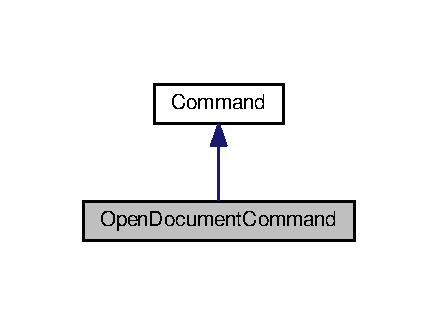
\includegraphics[width=210pt]{class_open_document_command__inherit__graph}
\end{center}
\end{figure}


Collaboration diagram for Open\-Document\-Command\-:
\nopagebreak
\begin{figure}[H]
\begin{center}
\leavevmode
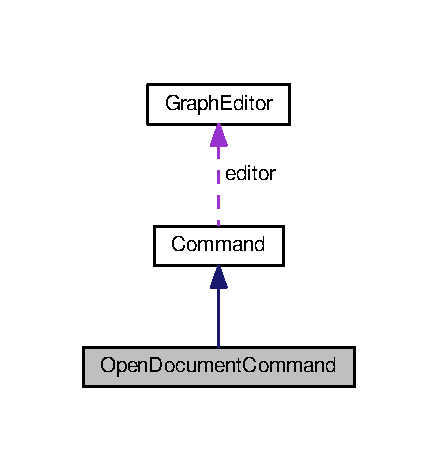
\includegraphics[width=210pt]{class_open_document_command__coll__graph}
\end{center}
\end{figure}
\subsection*{Public Member Functions}
\begin{DoxyCompactItemize}
\item 
\hyperlink{class_open_document_command_a7941657418acd57b98b52e858e98d3ed}{Open\-Document\-Command} (\hyperlink{class_graph_editor}{Graph\-Editor} $\ast$g, std\-::string doc\-\_\-name)
\item 
void \hyperlink{class_open_document_command_a80a9aa7d2c61e149c87800998f22f0ea}{execute} () override
\end{DoxyCompactItemize}
\subsection*{Additional Inherited Members}


\subsection{Constructor \& Destructor Documentation}
\hypertarget{class_open_document_command_a7941657418acd57b98b52e858e98d3ed}{\index{Open\-Document\-Command@{Open\-Document\-Command}!Open\-Document\-Command@{Open\-Document\-Command}}
\index{Open\-Document\-Command@{Open\-Document\-Command}!OpenDocumentCommand@{Open\-Document\-Command}}
\subsubsection[{Open\-Document\-Command}]{\setlength{\rightskip}{0pt plus 5cm}Open\-Document\-Command\-::\-Open\-Document\-Command (
\begin{DoxyParamCaption}
\item[{{\bf Graph\-Editor} $\ast$}]{g, }
\item[{std\-::string}]{doc\-\_\-name}
\end{DoxyParamCaption}
)\hspace{0.3cm}{\ttfamily [inline]}}}\label{class_open_document_command_a7941657418acd57b98b52e858e98d3ed}


\subsection{Member Function Documentation}
\hypertarget{class_open_document_command_a80a9aa7d2c61e149c87800998f22f0ea}{\index{Open\-Document\-Command@{Open\-Document\-Command}!execute@{execute}}
\index{execute@{execute}!OpenDocumentCommand@{Open\-Document\-Command}}
\subsubsection[{execute}]{\setlength{\rightskip}{0pt plus 5cm}void Open\-Document\-Command\-::execute (
\begin{DoxyParamCaption}
{}
\end{DoxyParamCaption}
)\hspace{0.3cm}{\ttfamily [inline]}, {\ttfamily [override]}, {\ttfamily [virtual]}}}\label{class_open_document_command_a80a9aa7d2c61e149c87800998f22f0ea}


Implements \hyperlink{class_command_a6fd7d9bd8df8bfc881e4d6c7cd1878b7}{Command}.



The documentation for this class was generated from the following file\-:\begin{DoxyCompactItemize}
\item 
\hyperlink{main_8cpp}{main.\-cpp}\end{DoxyCompactItemize}

\hypertarget{class_rectangle}{\section{Rectangle Class Reference}
\label{class_rectangle}\index{Rectangle@{Rectangle}}
}


{\ttfamily \#include $<$shape.\-h$>$}



Inheritance diagram for Rectangle\-:
\nopagebreak
\begin{figure}[H]
\begin{center}
\leavevmode
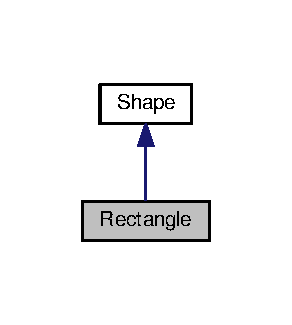
\includegraphics[width=140pt]{class_rectangle__inherit__graph}
\end{center}
\end{figure}


Collaboration diagram for Rectangle\-:
\nopagebreak
\begin{figure}[H]
\begin{center}
\leavevmode
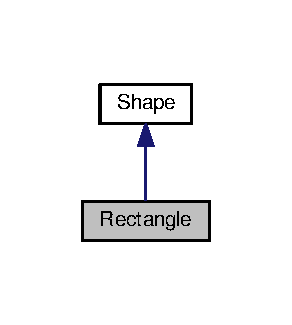
\includegraphics[width=140pt]{class_rectangle__coll__graph}
\end{center}
\end{figure}
\subsection*{Public Member Functions}
\begin{DoxyCompactItemize}
\item 
\hyperlink{class_rectangle}{Rectangle} \& \hyperlink{class_rectangle_af1e26c0d05ccdd77e45c1419b787a72c}{Create} () override
\item 
void \hyperlink{class_rectangle_a419cdba60fc01d44c9e793d1dad67d54}{Delete} () override
\end{DoxyCompactItemize}
\subsection*{Additional Inherited Members}


\subsection{Member Function Documentation}
\hypertarget{class_rectangle_af1e26c0d05ccdd77e45c1419b787a72c}{\index{Rectangle@{Rectangle}!Create@{Create}}
\index{Create@{Create}!Rectangle@{Rectangle}}
\subsubsection[{Create}]{\setlength{\rightskip}{0pt plus 5cm}{\bf Rectangle}\& Rectangle\-::\-Create (
\begin{DoxyParamCaption}
{}
\end{DoxyParamCaption}
)\hspace{0.3cm}{\ttfamily [inline]}, {\ttfamily [override]}, {\ttfamily [virtual]}}}\label{class_rectangle_af1e26c0d05ccdd77e45c1419b787a72c}


Implements \hyperlink{class_shape_ad2be0ce227fb05dcfec2691a671c82b5}{Shape}.

\hypertarget{class_rectangle_a419cdba60fc01d44c9e793d1dad67d54}{\index{Rectangle@{Rectangle}!Delete@{Delete}}
\index{Delete@{Delete}!Rectangle@{Rectangle}}
\subsubsection[{Delete}]{\setlength{\rightskip}{0pt plus 5cm}void Rectangle\-::\-Delete (
\begin{DoxyParamCaption}
{}
\end{DoxyParamCaption}
)\hspace{0.3cm}{\ttfamily [inline]}, {\ttfamily [override]}, {\ttfamily [virtual]}}}\label{class_rectangle_a419cdba60fc01d44c9e793d1dad67d54}


Implements \hyperlink{class_shape_a03a2b4615053e0a0edbdc42283e0bb04}{Shape}.



The documentation for this class was generated from the following file\-:\begin{DoxyCompactItemize}
\item 
\hyperlink{shape_8h}{shape.\-h}\end{DoxyCompactItemize}

\hypertarget{class_save_as_document_command}{\section{Save\-As\-Document\-Command Class Reference}
\label{class_save_as_document_command}\index{Save\-As\-Document\-Command@{Save\-As\-Document\-Command}}
}


Inheritance diagram for Save\-As\-Document\-Command\-:
\nopagebreak
\begin{figure}[H]
\begin{center}
\leavevmode
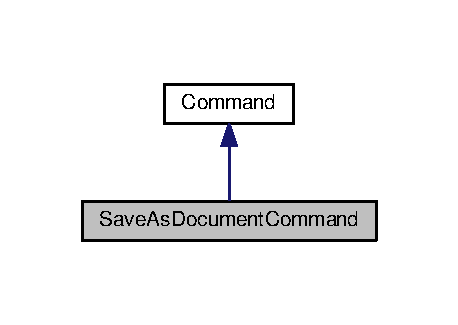
\includegraphics[width=220pt]{class_save_as_document_command__inherit__graph}
\end{center}
\end{figure}


Collaboration diagram for Save\-As\-Document\-Command\-:
\nopagebreak
\begin{figure}[H]
\begin{center}
\leavevmode
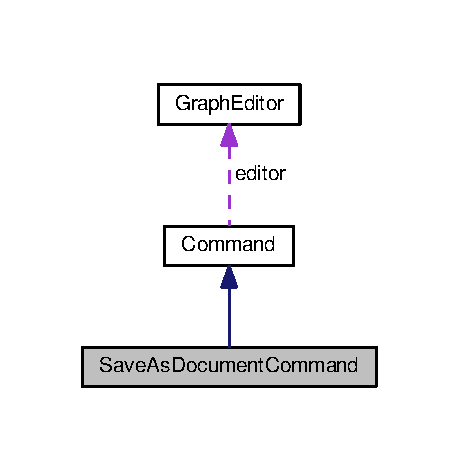
\includegraphics[width=220pt]{class_save_as_document_command__coll__graph}
\end{center}
\end{figure}
\subsection*{Public Member Functions}
\begin{DoxyCompactItemize}
\item 
\hyperlink{class_save_as_document_command_af1ee9a34336f4831a1a72f1aabaebf13}{Save\-As\-Document\-Command} (\hyperlink{class_graph_editor}{Graph\-Editor} $\ast$g, std\-::string doc\-\_\-name)
\item 
void \hyperlink{class_save_as_document_command_a7e24e4880ba0d3545f3df16ef5116d40}{execute} () override
\end{DoxyCompactItemize}
\subsection*{Additional Inherited Members}


\subsection{Constructor \& Destructor Documentation}
\hypertarget{class_save_as_document_command_af1ee9a34336f4831a1a72f1aabaebf13}{\index{Save\-As\-Document\-Command@{Save\-As\-Document\-Command}!Save\-As\-Document\-Command@{Save\-As\-Document\-Command}}
\index{Save\-As\-Document\-Command@{Save\-As\-Document\-Command}!SaveAsDocumentCommand@{Save\-As\-Document\-Command}}
\subsubsection[{Save\-As\-Document\-Command}]{\setlength{\rightskip}{0pt plus 5cm}Save\-As\-Document\-Command\-::\-Save\-As\-Document\-Command (
\begin{DoxyParamCaption}
\item[{{\bf Graph\-Editor} $\ast$}]{g, }
\item[{std\-::string}]{doc\-\_\-name}
\end{DoxyParamCaption}
)\hspace{0.3cm}{\ttfamily [inline]}}}\label{class_save_as_document_command_af1ee9a34336f4831a1a72f1aabaebf13}


\subsection{Member Function Documentation}
\hypertarget{class_save_as_document_command_a7e24e4880ba0d3545f3df16ef5116d40}{\index{Save\-As\-Document\-Command@{Save\-As\-Document\-Command}!execute@{execute}}
\index{execute@{execute}!SaveAsDocumentCommand@{Save\-As\-Document\-Command}}
\subsubsection[{execute}]{\setlength{\rightskip}{0pt plus 5cm}void Save\-As\-Document\-Command\-::execute (
\begin{DoxyParamCaption}
{}
\end{DoxyParamCaption}
)\hspace{0.3cm}{\ttfamily [inline]}, {\ttfamily [override]}, {\ttfamily [virtual]}}}\label{class_save_as_document_command_a7e24e4880ba0d3545f3df16ef5116d40}


Implements \hyperlink{class_command_a6fd7d9bd8df8bfc881e4d6c7cd1878b7}{Command}.



The documentation for this class was generated from the following file\-:\begin{DoxyCompactItemize}
\item 
\hyperlink{main_8cpp}{main.\-cpp}\end{DoxyCompactItemize}

\hypertarget{class_save_document_command}{\section{Save\-Document\-Command Class Reference}
\label{class_save_document_command}\index{Save\-Document\-Command@{Save\-Document\-Command}}
}


Inheritance diagram for Save\-Document\-Command\-:
\nopagebreak
\begin{figure}[H]
\begin{center}
\leavevmode
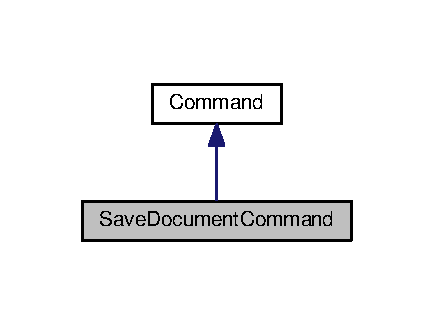
\includegraphics[width=208pt]{class_save_document_command__inherit__graph}
\end{center}
\end{figure}


Collaboration diagram for Save\-Document\-Command\-:
\nopagebreak
\begin{figure}[H]
\begin{center}
\leavevmode
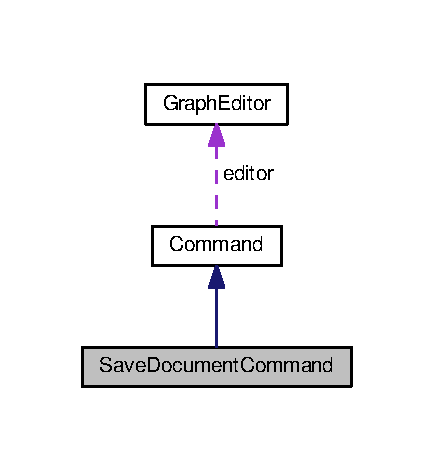
\includegraphics[width=208pt]{class_save_document_command__coll__graph}
\end{center}
\end{figure}
\subsection*{Public Member Functions}
\begin{DoxyCompactItemize}
\item 
\hyperlink{class_save_document_command_a3d51437ea555c31053bc10457393e565}{Save\-Document\-Command} (\hyperlink{class_graph_editor}{Graph\-Editor} $\ast$g)
\item 
void \hyperlink{class_save_document_command_a2c3e0a729f64b2577ed201cf20395895}{execute} () override
\end{DoxyCompactItemize}
\subsection*{Additional Inherited Members}


\subsection{Constructor \& Destructor Documentation}
\hypertarget{class_save_document_command_a3d51437ea555c31053bc10457393e565}{\index{Save\-Document\-Command@{Save\-Document\-Command}!Save\-Document\-Command@{Save\-Document\-Command}}
\index{Save\-Document\-Command@{Save\-Document\-Command}!SaveDocumentCommand@{Save\-Document\-Command}}
\subsubsection[{Save\-Document\-Command}]{\setlength{\rightskip}{0pt plus 5cm}Save\-Document\-Command\-::\-Save\-Document\-Command (
\begin{DoxyParamCaption}
\item[{{\bf Graph\-Editor} $\ast$}]{g}
\end{DoxyParamCaption}
)\hspace{0.3cm}{\ttfamily [inline]}}}\label{class_save_document_command_a3d51437ea555c31053bc10457393e565}


\subsection{Member Function Documentation}
\hypertarget{class_save_document_command_a2c3e0a729f64b2577ed201cf20395895}{\index{Save\-Document\-Command@{Save\-Document\-Command}!execute@{execute}}
\index{execute@{execute}!SaveDocumentCommand@{Save\-Document\-Command}}
\subsubsection[{execute}]{\setlength{\rightskip}{0pt plus 5cm}void Save\-Document\-Command\-::execute (
\begin{DoxyParamCaption}
{}
\end{DoxyParamCaption}
)\hspace{0.3cm}{\ttfamily [inline]}, {\ttfamily [override]}, {\ttfamily [virtual]}}}\label{class_save_document_command_a2c3e0a729f64b2577ed201cf20395895}


Implements \hyperlink{class_command_a6fd7d9bd8df8bfc881e4d6c7cd1878b7}{Command}.



The documentation for this class was generated from the following file\-:\begin{DoxyCompactItemize}
\item 
\hyperlink{main_8cpp}{main.\-cpp}\end{DoxyCompactItemize}

\hypertarget{class_shape}{\section{Shape Class Reference}
\label{class_shape}\index{Shape@{Shape}}
}


{\ttfamily \#include $<$shape.\-h$>$}



Inheritance diagram for Shape\-:
\nopagebreak
\begin{figure}[H]
\begin{center}
\leavevmode
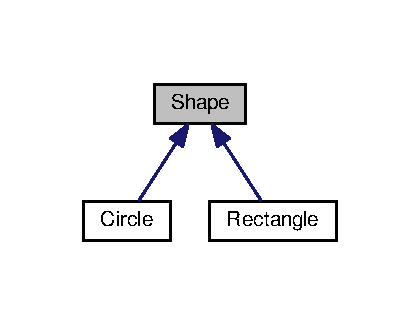
\includegraphics[width=201pt]{class_shape__inherit__graph}
\end{center}
\end{figure}
\subsection*{Public Member Functions}
\begin{DoxyCompactItemize}
\item 
virtual \hyperlink{class_shape_ac8ad2fd02e1e94beeb98e65ab795cd56}{$\sim$\-Shape} ()=default
\item 
virtual \hyperlink{class_shape}{Shape} \& \hyperlink{class_shape_ad2be0ce227fb05dcfec2691a671c82b5}{Create} ()=0
\item 
virtual void \hyperlink{class_shape_a03a2b4615053e0a0edbdc42283e0bb04}{Delete} ()=0
\end{DoxyCompactItemize}
\subsection*{Protected Member Functions}
\begin{DoxyCompactItemize}
\item 
\hyperlink{class_shape_adfc1f3a9555c8e8ef174f84909ec6a47}{Shape} ()=default
\end{DoxyCompactItemize}


\subsection{Constructor \& Destructor Documentation}
\hypertarget{class_shape_ac8ad2fd02e1e94beeb98e65ab795cd56}{\index{Shape@{Shape}!$\sim$\-Shape@{$\sim$\-Shape}}
\index{$\sim$\-Shape@{$\sim$\-Shape}!Shape@{Shape}}
\subsubsection[{$\sim$\-Shape}]{\setlength{\rightskip}{0pt plus 5cm}virtual Shape\-::$\sim$\-Shape (
\begin{DoxyParamCaption}
{}
\end{DoxyParamCaption}
)\hspace{0.3cm}{\ttfamily [virtual]}, {\ttfamily [default]}}}\label{class_shape_ac8ad2fd02e1e94beeb98e65ab795cd56}
\hypertarget{class_shape_adfc1f3a9555c8e8ef174f84909ec6a47}{\index{Shape@{Shape}!Shape@{Shape}}
\index{Shape@{Shape}!Shape@{Shape}}
\subsubsection[{Shape}]{\setlength{\rightskip}{0pt plus 5cm}Shape\-::\-Shape (
\begin{DoxyParamCaption}
{}
\end{DoxyParamCaption}
)\hspace{0.3cm}{\ttfamily [protected]}, {\ttfamily [default]}}}\label{class_shape_adfc1f3a9555c8e8ef174f84909ec6a47}


\subsection{Member Function Documentation}
\hypertarget{class_shape_ad2be0ce227fb05dcfec2691a671c82b5}{\index{Shape@{Shape}!Create@{Create}}
\index{Create@{Create}!Shape@{Shape}}
\subsubsection[{Create}]{\setlength{\rightskip}{0pt plus 5cm}virtual {\bf Shape}\& Shape\-::\-Create (
\begin{DoxyParamCaption}
{}
\end{DoxyParamCaption}
)\hspace{0.3cm}{\ttfamily [pure virtual]}}}\label{class_shape_ad2be0ce227fb05dcfec2691a671c82b5}


Implemented in \hyperlink{class_rectangle_af1e26c0d05ccdd77e45c1419b787a72c}{Rectangle}, and \hyperlink{class_circle_acbb38b1159540be80700263d78a9805e}{Circle}.

\hypertarget{class_shape_a03a2b4615053e0a0edbdc42283e0bb04}{\index{Shape@{Shape}!Delete@{Delete}}
\index{Delete@{Delete}!Shape@{Shape}}
\subsubsection[{Delete}]{\setlength{\rightskip}{0pt plus 5cm}virtual void Shape\-::\-Delete (
\begin{DoxyParamCaption}
{}
\end{DoxyParamCaption}
)\hspace{0.3cm}{\ttfamily [pure virtual]}}}\label{class_shape_a03a2b4615053e0a0edbdc42283e0bb04}


Implemented in \hyperlink{class_rectangle_a419cdba60fc01d44c9e793d1dad67d54}{Rectangle}, and \hyperlink{class_circle_aef290a1d0349f56cb01884b6735042cb}{Circle}.



The documentation for this class was generated from the following file\-:\begin{DoxyCompactItemize}
\item 
\hyperlink{shape_8h}{shape.\-h}\end{DoxyCompactItemize}

\chapter{File Documentation}
\hypertarget{document_8h}{\section{document.\-h File Reference}
\label{document_8h}\index{document.\-h@{document.\-h}}
}
{\ttfamily \#include \char`\"{}shape.\-h\char`\"{}}\\*
{\ttfamily \#include $<$iostream$>$}\\*
Include dependency graph for document.\-h\-:
\nopagebreak
\begin{figure}[H]
\begin{center}
\leavevmode
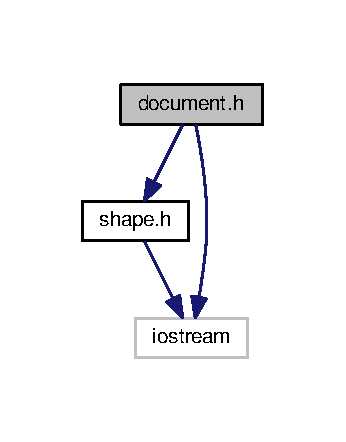
\includegraphics[width=166pt]{document_8h__incl}
\end{center}
\end{figure}
This graph shows which files directly or indirectly include this file\-:
\nopagebreak
\begin{figure}[H]
\begin{center}
\leavevmode
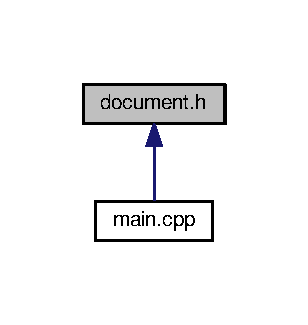
\includegraphics[width=148pt]{document_8h__dep__incl}
\end{center}
\end{figure}
\subsection*{Classes}
\begin{DoxyCompactItemize}
\item 
class \hyperlink{class_document}{Document}
\end{DoxyCompactItemize}

\hypertarget{main_8cpp}{\section{main.\-cpp File Reference}
\label{main_8cpp}\index{main.\-cpp@{main.\-cpp}}
}
{\ttfamily \#include $<$iostream$>$}\\*
{\ttfamily \#include $<$utility$>$}\\*
{\ttfamily \#include $<$tuple$>$}\\*
{\ttfamily \#include $<$bitset$>$}\\*
{\ttfamily \#include $<$vector$>$}\\*
{\ttfamily \#include $<$list$>$}\\*
{\ttfamily \#include $<$functional$>$}\\*
{\ttfamily \#include \char`\"{}check\-\_\-type.\-h\char`\"{}}\\*
{\ttfamily \#include \char`\"{}print\-\_\-tuple.\-h\char`\"{}}\\*
Include dependency graph for main.\-cpp\-:
\nopagebreak
\begin{figure}[H]
\begin{center}
\leavevmode
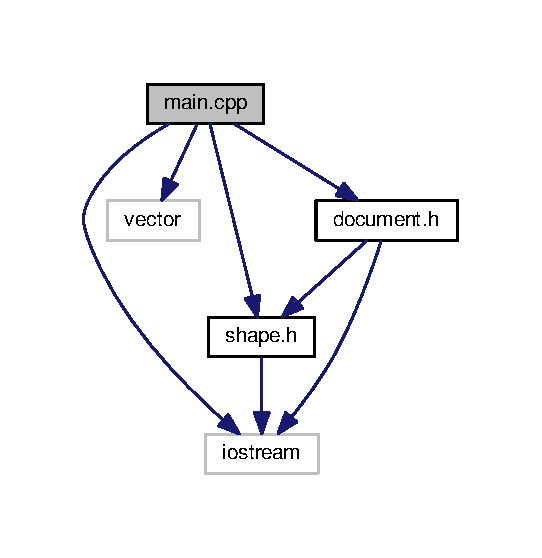
\includegraphics[width=350pt]{main_8cpp__incl}
\end{center}
\end{figure}
\subsection*{Classes}
\begin{DoxyCompactItemize}
\item 
struct \hyperlink{structprinter}{printer}
\end{DoxyCompactItemize}
\subsection*{Functions}
\begin{DoxyCompactItemize}
\item 
{\footnotesize template$<$typename T , typename Printer $>$ }\\void \hyperlink{main_8cpp_a2e507a49231a92dd51a74153d941a10b}{print} (T \&\&t, Printer \hyperlink{structprinter}{printer}, int)
\item 
{\footnotesize template$<$typename T , typename Printer $>$ }\\void \hyperlink{main_8cpp_a4d92f34c852cf08c698ce9ff9b8f40e1}{print} (T \&\&t, Printer \hyperlink{structprinter}{printer}, char)
\item 
{\footnotesize template$<$typename Printer $>$ }\\void \hyperlink{main_8cpp_a650caaec23d14a266eb863256c192da2}{print} (std\-::string t, Printer, char)
\item 
{\footnotesize template$<$typename T $>$ }\\void \hyperlink{main_8cpp_a5a2ed2f3cccd43a84bfd7d2740475be1}{print\-\_\-ip} (T \&\&t)
\item 
{\footnotesize template$<$typename... Args$>$ }\\void \hyperlink{main_8cpp_adf6cb0a6bc6c2be1c8468b73110978ba}{print\-\_\-ip} (std\-::tuple$<$ Args...$>$ t)
\item 
int \hyperlink{main_8cpp_ae66f6b31b5ad750f1fe042a706a4e3d4}{main} ()
\end{DoxyCompactItemize}


\subsection{Function Documentation}
\hypertarget{main_8cpp_ae66f6b31b5ad750f1fe042a706a4e3d4}{\index{main.\-cpp@{main.\-cpp}!main@{main}}
\index{main@{main}!main.cpp@{main.\-cpp}}
\subsubsection[{main}]{\setlength{\rightskip}{0pt plus 5cm}int main (
\begin{DoxyParamCaption}
{}
\end{DoxyParamCaption}
)}}\label{main_8cpp_ae66f6b31b5ad750f1fe042a706a4e3d4}
\hypertarget{main_8cpp_a2e507a49231a92dd51a74153d941a10b}{\index{main.\-cpp@{main.\-cpp}!print@{print}}
\index{print@{print}!main.cpp@{main.\-cpp}}
\subsubsection[{print}]{\setlength{\rightskip}{0pt plus 5cm}template$<$typename T , typename Printer $>$ void print (
\begin{DoxyParamCaption}
\item[{T \&\&}]{t, }
\item[{Printer}]{printer, }
\item[{int}]{}
\end{DoxyParamCaption}
)}}\label{main_8cpp_a2e507a49231a92dd51a74153d941a10b}
Обработка целочисленных типов 
\begin{DoxyParams}[1]{Parameters}
\mbox{\tt in}  & {\em T\&\&} & Объект, который нужно обработать \\
\hline
\mbox{\tt in}  & {\em int} & -\/ целочисленный тип \\
\hline
\end{DoxyParams}
\hypertarget{main_8cpp_a4d92f34c852cf08c698ce9ff9b8f40e1}{\index{main.\-cpp@{main.\-cpp}!print@{print}}
\index{print@{print}!main.cpp@{main.\-cpp}}
\subsubsection[{print}]{\setlength{\rightskip}{0pt plus 5cm}template$<$typename T , typename Printer $>$ void print (
\begin{DoxyParamCaption}
\item[{T \&\&}]{t, }
\item[{Printer}]{printer, }
\item[{char}]{}
\end{DoxyParamCaption}
)}}\label{main_8cpp_a4d92f34c852cf08c698ce9ff9b8f40e1}
Обработка контейнерных типов 
\begin{DoxyParams}[1]{Parameters}
\mbox{\tt in}  & {\em T\&\&} & Объект, который нужно обработать \\
\hline
\mbox{\tt in}  & {\em char} & -\/ контейнерный тип \\
\hline
\end{DoxyParams}
\hypertarget{main_8cpp_a650caaec23d14a266eb863256c192da2}{\index{main.\-cpp@{main.\-cpp}!print@{print}}
\index{print@{print}!main.cpp@{main.\-cpp}}
\subsubsection[{print}]{\setlength{\rightskip}{0pt plus 5cm}template$<$typename Printer $>$ void print (
\begin{DoxyParamCaption}
\item[{std\-::string}]{t, }
\item[{Printer}]{, }
\item[{char}]{}
\end{DoxyParamCaption}
)}}\label{main_8cpp_a650caaec23d14a266eb863256c192da2}
Обработка строк 
\begin{DoxyParams}[1]{Parameters}
\mbox{\tt in}  & {\em std\-::string} & строка, которую нужно обработать \\
\hline
\mbox{\tt in}  & {\em int} & -\/ char -\/ контейнерный тип \\
\hline
\end{DoxyParams}
\hypertarget{main_8cpp_a5a2ed2f3cccd43a84bfd7d2740475be1}{\index{main.\-cpp@{main.\-cpp}!print\-\_\-ip@{print\-\_\-ip}}
\index{print\-\_\-ip@{print\-\_\-ip}!main.cpp@{main.\-cpp}}
\subsubsection[{print\-\_\-ip}]{\setlength{\rightskip}{0pt plus 5cm}template$<$typename T $>$ void print\-\_\-ip (
\begin{DoxyParamCaption}
\item[{T \&\&}]{t}
\end{DoxyParamCaption}
)}}\label{main_8cpp_a5a2ed2f3cccd43a84bfd7d2740475be1}
Отделяет контейнеры от целочисленных типов 
\begin{DoxyParams}[1]{Parameters}
\mbox{\tt in}  & {\em T\&\&} & Объект, который нужно обработать \\
\hline
\end{DoxyParams}
\hypertarget{main_8cpp_adf6cb0a6bc6c2be1c8468b73110978ba}{\index{main.\-cpp@{main.\-cpp}!print\-\_\-ip@{print\-\_\-ip}}
\index{print\-\_\-ip@{print\-\_\-ip}!main.cpp@{main.\-cpp}}
\subsubsection[{print\-\_\-ip}]{\setlength{\rightskip}{0pt plus 5cm}template$<$typename... Args$>$ void print\-\_\-ip (
\begin{DoxyParamCaption}
\item[{std\-::tuple$<$ Args...$>$}]{t}
\end{DoxyParamCaption}
)}}\label{main_8cpp_adf6cb0a6bc6c2be1c8468b73110978ba}
Отдельная специализация для кортежа 
\hypertarget{shape_8h}{\section{shape.\-h File Reference}
\label{shape_8h}\index{shape.\-h@{shape.\-h}}
}
{\ttfamily \#include $<$iostream$>$}\\*
Include dependency graph for shape.\-h\-:
\nopagebreak
\begin{figure}[H]
\begin{center}
\leavevmode
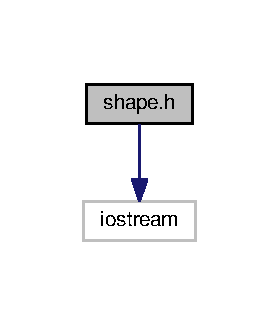
\includegraphics[width=134pt]{shape_8h__incl}
\end{center}
\end{figure}
This graph shows which files directly or indirectly include this file\-:
\nopagebreak
\begin{figure}[H]
\begin{center}
\leavevmode
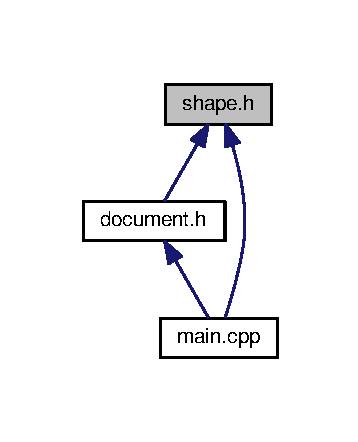
\includegraphics[width=172pt]{shape_8h__dep__incl}
\end{center}
\end{figure}
\subsection*{Classes}
\begin{DoxyCompactItemize}
\item 
class \hyperlink{class_shape}{Shape}
\item 
class \hyperlink{class_circle}{Circle}
\item 
class \hyperlink{class_rectangle}{Rectangle}
\end{DoxyCompactItemize}

\hypertarget{version_8h}{\section{version.\-h File Reference}
\label{version_8h}\index{version.\-h@{version.\-h}}
}
\subsection*{Macros}
\begin{DoxyCompactItemize}
\item 
\#define \hyperlink{version_8h_a4a5fc96a4bdd7d68ed99ccce9ca2e77e}{P\-R\-O\-J\-E\-C\-T\-\_\-\-V\-E\-R\-S\-I\-O\-N\-\_\-\-P\-A\-T\-C\-H}~36
\end{DoxyCompactItemize}


\subsection{Macro Definition Documentation}
\hypertarget{version_8h_a4a5fc96a4bdd7d68ed99ccce9ca2e77e}{\index{version.\-h@{version.\-h}!P\-R\-O\-J\-E\-C\-T\-\_\-\-V\-E\-R\-S\-I\-O\-N\-\_\-\-P\-A\-T\-C\-H@{P\-R\-O\-J\-E\-C\-T\-\_\-\-V\-E\-R\-S\-I\-O\-N\-\_\-\-P\-A\-T\-C\-H}}
\index{P\-R\-O\-J\-E\-C\-T\-\_\-\-V\-E\-R\-S\-I\-O\-N\-\_\-\-P\-A\-T\-C\-H@{P\-R\-O\-J\-E\-C\-T\-\_\-\-V\-E\-R\-S\-I\-O\-N\-\_\-\-P\-A\-T\-C\-H}!version.h@{version.\-h}}
\subsubsection[{P\-R\-O\-J\-E\-C\-T\-\_\-\-V\-E\-R\-S\-I\-O\-N\-\_\-\-P\-A\-T\-C\-H}]{\setlength{\rightskip}{0pt plus 5cm}\#define P\-R\-O\-J\-E\-C\-T\-\_\-\-V\-E\-R\-S\-I\-O\-N\-\_\-\-P\-A\-T\-C\-H~36}}\label{version_8h_a4a5fc96a4bdd7d68ed99ccce9ca2e77e}

%--- End generated contents ---

% Index
\newpage
\phantomsection
\addcontentsline{toc}{chapter}{Index}
\printindex

\end{document}
